\documentclass[a4paper,11pt]{article}
\usepackage[margin=1in]{geometry}
\usepackage{fontspec}
\setmainfont{Times New Roman}
\setsansfont{Arial}
\setmonofont{Consolas}[Scale=0.85]
\usepackage[english,russian]{babel}
\usepackage{amsmath,amssymb,amsthm,graphicx,booktabs}
\usepackage[hidelinks]{hyperref}
\setlength{\emergencystretch}{3em}
\hypersetup{pdftitle={Сертификатные оценки метода Франка–Вульфа с обратным поиском при кривизне, зависящей от значения функции},pdfauthor={Yaroslav P. Lyakhov and Stepan Suvorov}}
\newtheorem{theorem}{Теорема}[section]
\newtheorem{lemma}[theorem]{Лемма}
\newtheorem{proposition}[theorem]{Утверждение}
\newtheorem{corollary}[theorem]{Следствие}
\newcommand{\norm}[1]{\left\|#1\right\|}
\newcommand{\inner}[2]{\left\langle#1,#2\right\rangle}
\newcommand{\R}{\mathbb R}
\newcommand{\ceil}[1]{\left\lceil#1\right\rceil}
\DeclareMathOperator{\artanh}{artanh}
\title{Сертификатные оценки метода Франка–Вульфа\\с обратным поиском при кривизне,\\зависящей от значения функции}
\author{Yaroslav P. Lyakhov \and Stepan Suvorov}
\date{17 октября 2026 г.}
\begin{document}
\maketitle
\begin{abstract}
Рассматривается выпуклая минимизация на компактном выпуклом множестве,
когда норма гессиана ограничена величиной $H_0+H_1(f-f_Q^*)$, где
$f_Q^*$ — минимум на допустимом множестве. Для обычного метода
Франка–Вульфа с квадратичным обратным поиском доказана оценка
$O(H_0D^2/\varepsilon+(1+H_1D^2)\log(U_0/\varepsilon))$ числа
обновлений до достижения наблюдаемого сертификата точности с отдельным
явным слагаемым инициализации. Метод не получает ни параметров кривизны,
ни оптимального значения. Фазовый аргумент контролирует оценки,
запаздывающие относительно убывающей локальной кривизны. После $N$
обновлений число всех пробных вычислений функции не превышает $1+2N$
плюс явная логарифмическая добавка. Стандартные шаги удаления наследуют
выпуклую оценку. При геометрическом условии оценки ошибки они дают
логарифмическую зависимость от сертификатной точности с отдельным вкладом
начальной кривизны. Дифференциальное сравнение даёт оптимальную поточечную
верхнюю огибающую зазора Франка–Вульфа и достигающие её одномерные
функции. При $H_0=0$ множество решений является экспонированной гранью,
на которой градиент постоянен; метод Франка–Вульфа с шагами удаления и
обратным поиском достигает точного оптимума за конечное число обновлений
без дополнительной гипотезы геометрического роста. Квадратичный
контрпример отделяет этот предельный случай от любого $H_0>0$.
Точная минимизация на отрезке и короткие шаги с известной кривизной
служат вариантами сравнения в той же модели линейного оракула.
Контролируемые эксперименты с аналитически проверенными функциями и
реальными пуассоновскими данными разделяют влияние инициализации,
геометрии активной грани и стоимости остановки. Они не выявляют
универсального преимущества инициализации по сертификату и показывают
режимы, в которых скалярный сертификат существенно запаздывает
относительно точности по функции. Результаты относятся к существующему
методу обратного поиска; новый алгоритм и оптимальная оракульная
сложность не устанавливаются.
\end{abstract}
\section{Введение}
Методы Франка–Вульфа (FW) решают линейные подзадачи вместо вычисления
проекций. Обратный поиск позволяет применять квадратичные модели шага
без заранее заданной константы гладкости, а шаги удаления улучшают
продвижение на многогранниках~\cite{braun,pedregosa,lacostejaggi}.
Однако глобальная граница кривизны может терять существенную информацию,
когда кривизна убывает вместе со значением целевой функции.
Мы рассматриваем аффинное ограничение гессиана через отклонение потерь
от оптимума, изученное в~\cite{warmup}, применительно к выпуклой задаче
с ограничениями. Оно также является случаем показателя один в семействе
гладкости, зависящей от потерь, из~\cite{liuwarmup}.
Более общие ограничения гессиана через значение функции
ранее возникли в теориях самоограничивающейся
регулярности~\cite{kale,caoselfbound}; само условие не является
вкладом настоящей работы.

Наш вопрос количественный: что гарантирует обычный обратный поиск
для наблюдаемого правила остановки при таком условии, с учётом
начальной оценки и всех пробных вычислений? Теорема~\ref{thm:fw}
отвечает на него, разделяя вклады $H_0/\varepsilon$ и
$H_1\log(1/\varepsilon)$. Основной инструмент — потенциал оценок,
которые остаются слишком большими при переходе сертификата на более
низкие двоичные уровни. Он не меняет алгоритм и не ограничивает LMO
множеством подуровня. Теорема~\ref{thm:afw} переносит результат с
помощью стандартного подсчёта удаляемых атомов. При геометрическом
неравенстве для зазора теорема~\ref{thm:geometric} даёт логарифмическую
зависимость от точности с явной начальной ценой $H_1$.
Теорема~\ref{lem:bridge} устанавливает оптимальную поточечную огибающую
FW-зазора для этого класса и одномерные функции, на которых она
достигается. Утверждение~\ref{prop:zeroface} характеризует случай
$H_0=0$: всё множество решений является экспонированной гранью с общим
градиентом. Теорема~\ref{thm:zerofinite} затем усиливает приближённую
остановку до конечного достижения точного оптимума методом AFW с
обратным поиском, с явной оценкой, не зависящей от запрошенной точности.
Используются известные механизмы идентификации~\cite{bomze,garber};
новый алгоритм AFW и общая теория идентификации не заявляются.
Приведены полные доказательства, граничные примеры и контрпримеры.

\paragraph{Связанные исследования.}
Гладкость, зависящая от функции, и двухрежимные оценки градиентных
методов предшествуют этой работе~\cite{warmup,lobanovkoloskova,lobanov}.
Выгузов и Стонякин~\cite{vyguzov} анализируют FW при гладкости,
зависящей от нормы градиента. На компактном выпуклом множестве
$f-f_Q^*\le D\norm{\nabla f}$ переводит наше условие в соответствующую
границу гессиана, но глобальная оценка максимального градиента не
сохраняет изучаемое здесь разделение зависимостей.
Pedregosa и соавторы~\cite[теоремы 1, 3 и 4]{pedregosa} уже дают
подсчёт проб обратного поиска, двойственную гарантию Фенхеля с
усреднённым градиентом и линейную сходимость AFW с принятыми локальными
оценками кривизны. Наш максимум скалярных нижних оценок отличается от
этой двойственной величины; их значения нельзя просто отождествить.
Наш результат специализирует локальную кривизну к порогу сертификата
и явно учитывает запаздывание. Приоритет обратного поиска, двойственных
сертификатов, линейной сходимости AFW и телескопического тождества для
отклонённых проб не заявляется.
Лучшие накопленные касательные границы и вычислимые зазоры остановки
также известны ранее~\cite[метод 1]{freundgrigas}. Оптимистический FW и
прямые-двойственные короткие шаги явно оптимизируют вычислимые зазоры
при глобальной гладкости~\cite[утверждение 4.1]{beyondshort}; они не
оценивают анализируемое здесь унаследованное правило деления и
умножения оценки на два.

К другим связанным подходам относятся FW для обобщённо
самосогласованных функций, адаптивные шаги Брегмана и адаптивный
слайдинг условного градиента~\cite{selfconcordant,bregmanfw,adcgs}.
Оценки расширенной кривизны и схемы с рестартами при условиях оценки
ошибки уже дают двухрежимные и геометрические скорости~\cite{wirth,restartfw};
линейная сходимость по функции и FW-зазору за пределами глобальной
гладкости градиента также известна для логарифмически однородных
барьеров~\cite{zhao}. Автоматически обусловленный FW служит практическим
вариантом сравнения с иной предварительной обработкой и учётом
оракулов~\cite{autoconditioned}. Инициализация по разности градиентов с
обратным поиском~\cite{khademi} и условный градиент без линейного
поиска~\cite{yagishita} дают другие способы адаптации к параметрам.
ALFCG оценивает гладкость без линейного поиска, но сохраняет условия
глобальной покомпонентной или средней гладкости и стохастический
критерий стационарности~\cite[раздел 3]{alfcg}.
Недавний Newton--FW с демпфированием использует информацию гессиана и
предполагает его положительную определённость~\cite[раздел 1]{newtonfw};
это не охватывает наш оптимум с нулевой базовой кривизной, где гессиан
обращается в нуль.
Приложение~\ref{app:comparison} уточняет используемые различия.
Прямая подстановка глобальной гладкости обычно слабее, но это не
означает, что эквивалентное следствие невозможно вывести из другого
адаптивного анализа.

Экспериментальная часть отвечает на три вопроса, существенных для
интерпретации оценок: помогает ли инициализация по сертификату независимо
от смены стартовой точки; устраняют ли шаги удаления препятствия
активной грани; означает ли отсутствие остановки оставшуюся ошибку по
функции или консервативность сертификата. Бюджеты оракулов учитываются
раздельно; неуспешные запуски сохраняются.

\section{Обычный обратный поиск и вычислимый сертификат}
\label{sec:model}
Пусть $Q\subset\R^d$ — непустое компактное выпуклое множество диаметра
$D>0$. Пусть $f$ выпукла и принадлежит $C^2$ в окрестности $Q$,
$f_Q^*=\min_Q f$ и $\delta(x)=f(x)-f_Q^*$. Предполагается, что
\begin{equation}\label{eq:curvature}
 \norm{\nabla^2f(z)}_2\le H_0+H_1\delta(z),\qquad z\in Q,
 \quad H_0,H_1\ge0.
\end{equation}
Опорное значение в этом условии — минимум на допустимом множестве.
Ограничение относительно меньшего безусловного инфимума не влечёт
того же ограничения относительно условного минимума без изменения
$H_0$. При $D=0$ единственная допустимая точка решает задачу.

В исходной точке $x_k$ вызывается точный оракул линейной минимизации
(LMO), после чего вычисляются FW-зазор и накопленный сертификат:
\begin{align}
 s_k&\in\arg\min_{v\in Q}\inner{\nabla f(x_k)}{v},\quad
 G_k=\inner{\nabla f(x_k)}{x_k-s_k},\label{eq:gap}\\
 \ell_k&=\max_{0\le i\le k}\{f(x_i)-G_i\},\quad
 U_k=f(x_k)-\ell_k.\label{eq:certificate}
\end{align}
Выпуклость даёт $0\le\delta_k\le U_k\le G_k$. Известную корректную
нижнюю границу можно включить в $\ell_k$, но она не обязательна.
Нулевой зазор удостоверяет оптимальность. Остановка происходит при
$U_k\le\varepsilon$.
Конструкция лучшей накопленной касательной границы известна ранее
\cite[метод 1, соглашение о максимизации]{freundgrigas}; новый анализ
касается её стоимости при зависящей от функции кривизне, а не самого
сертификата.

\paragraph{Алгоритм.}
Выберем $M>0$ и положим $L_{-1}=M$. В каждой нетерминальной исходной
точке зададим $d_k=s_k-x_k$, $q_k=\norm{d_k}$ и начнём с
$L=L_{k-1}/2$. Повторяем
\begin{equation}\label{eq:btstep}
 \alpha=\min\{1,G_k/(Lq_k^2)\},\qquad
 f(x_k+\alpha d_k)\le f(x_k)-\alpha G_k
                         +\tfrac12L\alpha^2q_k^2
\end{equation}
до выполнения неравенства, удваивая $L$ после каждого отказа.
Сохраняем $L_k=L$, обновляем $x_{k+1}=x_k+\alpha d_k$ и повторно
используем принятое значение функции. В ходе поиска заново вычисляются
лишь пробные значения функции. Это стандартная схема квадратичного
обратного поиска~\cite{pedregosa}. При фиксированном $M$ алгоритму не
нужны $D,H_0,H_1$ и $f_Q^*$. Необязательный выбор $M=U_0/D^2$
использует границу диаметра и первые оплаченные вызовы функции,
градиента и LMO.

\begin{lemma}[Локальная приёмка]\label{lem:local}
Для допустимого направления спуска $d$ с
$g=-\inner{\nabla f(x)}d>0$ и верхней границей шага $a_{\max}>0$
проверка~\eqref{eq:btstep} проходит для шага
\[
\alpha=\min\{a_{\max},g/(L\norm d^2)\},
\]
если
$L\ge H_0+H_1\delta(x)$. Любая принятая проба, независимо от этого
достаточного порога, удовлетворяет
\begin{equation}\label{eq:acceptedprogress}
 f(x)-f(x+\alpha d)\ge\tfrac12\alpha g.
\end{equation}
Следовательно, поиск завершается и
\begin{equation}\label{eq:localenvelope}
 L_k\le\max\{L_{k-1}/2,\ 2(H_0+H_1\delta_k)\}.
\end{equation}
Допускается также $a_{\max}>1$.
\end{lemma}
\begin{proof}
Запишем $h(t)=f(x+td)-f(x)$ и $K=H_0+H_1\delta(x)$.
Пока $h\le0$, ограничение гессиана даёт $h''(t)\le K\norm d^2$.
В начальный момент $h'(0)=-g<0$. При $K>0$ первый возврат к нулю
до $\min\{a_{\max},2g/(K\norm d^2)\}$ противоречит
$h(t)\le-gt+K\norm d^2t^2/2<0$. То же интегрирование доказывает
квадратичную верхнюю оценку вплоть до заданной пробы; при $K=0$
получается линейная верхняя модель. Её кривизна не превосходит $L$,
поэтому проверка проходит. Для любой принятой пробы
$L\alpha\norm d^2\le g$, откуда следует~\eqref{eq:acceptedprogress}.
Если был отказ, последняя отклонённая оценка меньше $K$, поэтому
принятая меньше $2K$; иначе она равна $L_{k-1}/2$.
\end{proof}

Таким образом, $f_k$ и $U_k$ не возрастают. В анализе используется
кривизна лишь на отрезке спуска, а не единая верхняя модель во всех
точках произвольного отрезка.

\begin{lemma}[Потенциал запаздывания]\label{lem:lag}
Пусть индексы фаз исходных точек не убывают и принадлежат
$\{0,\ldots,J-1\}$. Пусть положительные верхние границы удовлетворяют
$C_j/2\le C_{j+1}\le C_j$. Предположим, что обновление с $L_k>C_j$
в своей исходной фазе обязательно имеет $L_k=L_{k-1}/2$.
Тогда число таких запаздывающих обновлений не превышает
\[
 \ceil{\log_2\max\{1,M/C_0\}}+J-1.
\]
Утверждение применимо к любому префиксу и допускает пропуск начальных фаз.
\end{lemma}
\begin{proof}
Перед обновлением в фазе $j$ используем неотрицательный целочисленный
потенциал
\[
 p=\max\{0,\ceil{\log_2(L_{k-1}/C_j)}\}.
\]
Запаздывающее обновление уменьшает его на единицу; после незапаздывающего
обновления потенциал перед сменой фазы равен нулю. Переход вперёд
на $m$ фаз увеличивает его не более чем на $m$. От виртуальной
нулевой фазы сумма всех переходов, включая начальный, не превосходит
$J-1$. Неотрицательность даёт требуемый подсчёт.
\end{proof}

\begin{theorem}[Наблюдаемая остановка и полная стоимость функции]\label{thm:fw}
Для $0<\varepsilon<U_0$ положим
\[
 J=\ceil{\log_2(U_0/\varepsilon)},\qquad
 P=\ceil{\log_2\max\{1,MD^2/U_0\}}.
\]
Обычный обратный поиск достигает $U_N\le\varepsilon$ за
\begin{equation}\label{eq:fwcount}
 N\le P+\ceil{(6+16H_1D^2)J+32H_0D^2/\varepsilon}
\end{equation}
обновлений. Он использует $N+1$ градиентов и LMO, включая финальную
проверку. При фактическом $N\ge1$ все вычисления функции, включая
отклонённые пробы, учтены в оценке
\begin{equation}\label{eq:functioncount}
 N_f\le1+2N+\ceil{\log_2\max\{1,2(H_0+H_1U_0)/M\}}.
\end{equation}
При $N=0$ достаточно одного вычисления функции, градиента и LMO.
Оценки предполагают точные оракулы и точную арифметику.
\end{theorem}
\begin{proof}
Положим $b_j=U_0/2^j$ и отнесём нетерминальную исходную точку
к фазе $j$, если $b_j/2<U_k\le b_j$, где $j=0,\ldots,J-1$.
Используем
\[
 C_j=\max\{2(H_0+H_1b_j),\ b_j/(2D^2)\}.
\]
Эти границы убывают не более чем вдвое. По лемме~\ref{lem:local}
принятая оценка выше $C_j$ обязательно получена делением пополам
на первой пробе. Поскольку $C_0\ge U_0/(2D^2)$, лемма~\ref{lem:lag}
ограничивает число запаздывающих обновлений величиной $P+J$.

Для незапаздывающего обновления фазы $j$ неравенства
$G_k\ge U_k>b_j/2$ и $q_k\le D$ дают
\[
 f_k-f_{k+1}\ge p_j:=\min\{b_j/4,\ b_j^2/(8C_jD^2)\}.
\]
Каждое обновление уменьшает $f$, а суммарное уменьшение внутри фазы
не превосходит ошибки по функции в её начале, то есть не более $b_j$.
Поэтому число незапаздывающих обновлений фазы не превосходит
\[
 \lfloor b_j/p_j\rfloor+1
 \le5+16H_1D^2+16H_0D^2/b_j.
\]
Суммирование с использованием $\sum_{j<J}1/b_j<2/\varepsilon$
доказывает~\eqref{eq:fwcount}. Оценка ограничивает любой
незавершённый префикс, что также устанавливает остановку.

Локальная огибающая и монотонность $U$ дают
$L_k\le\max\{M/2^{k+1},2(H_0+H_1U_0)\}$.
Если $r_k$ — число отказов, то $L_k=2^{r_k-1}L_{k-1}$, поэтому
число вычисленных пробных значений в точности равно
\[
 \sum_{k<N}(r_k+1)=2N+\log_2(L_{N-1}/M).
\]
Добавляя начальное значение и используя огибающую, получаем
\eqref{eq:functioncount}. Принятые значения сохраняются.
\end{proof}

Последнее тождество стандартно~\cite{pedregosa}. При $M=U_0/D^2$
имеем $P=0$, а добавка к числу вычислений функции не зависит от
$\varepsilon$. Для порядка оценки эта нормировка необязательна.

\begin{proposition}[Инициализация заметна даже на аффинных функциях]
\label{prop:init}
Пусть $Q=[-1,1]$, $f(x)=-cx$, $c>0$, $x_0=-1$ и $L_{-1}=M>0$.
Для $0<\varepsilon<2c$ обратный поиск с делением пополам использует
ровно
\[
 N=\ceil{\log_2\left(1+\frac Mc(1-\varepsilon/(2c))\right)}
\]
обновлений. Следовательно, уменьшение $U_0$ вдвое может требовать
$\Theta(\log(M/c))$ обновлений.
\end{proposition}
\begin{proof}
Каждая проверка принимает первую пробу: $L_k=M/2^{k+1}$,
$x_{k+1}=\min\{1,x_k+c/L_k\}$. Касательная нижняя оценка всегда
равна $-c$, поэтому $x_N=\min\{1,-1+(2c/M)(2^N-1)\}$ и
$U_N=c(1-x_N)$. Решение неравенства остановки даёт формулу.
\end{proof}
Эта нижняя оценка относится к заданному правилу деления пополам,
а не к произвольным алгоритмам первого порядка.
При $M=U_0/D^2=c/2$ первый шаг решает задачу.

\paragraph{Сравнение с глобальной границей.}
Для $f(x)=\cosh(x)-1$ на $[-R,R]$ имеем $H_0=H_1=1$, тогда как
глобальная константа Липшица градиента равна $L_Q=\cosh R$.
При старте из $R$ получаем $U_0=2R\sinh R$. Для фиксированных
точности и $M$ наша оценка числа обновлений растёт как
$O(R^3+R^2/\varepsilon)$ при $R\to\infty$, в отличие от
экспоненциального слагаемого $L_QD^2/\varepsilon$, получаемого
подстановкой $H_0=L_Q,H_1=0$ в ту же сертификатную теорему.
Здесь сравниваются верхние оценки, а не время работы или оракульная
нижняя граница; точная минимизация на отрезке решает этот конкретный
одномерный пример за один шаг. Другие сравнения шагов приведены в
приложении~\ref{app:explicit}.

\section{Шаги удаления и геометрическое продвижение}
Пусть $Q=\operatorname{conv}(\mathcal A)$ для конечного множества
атомов. Поддерживается представление $x=\sum_{a\in S}\lambda_a a$
с положительными весами, сумма которых равна единице. Помимо полного
FW-атома $s$, выбирается
$v\in\arg\max_{a\in S}\inner{\nabla f(x)}a$.
Из направлений $s-x$ и $x-v$ используется направление с большим
зазором; при равенстве выбирается FW. Его зазор $g$ удовлетворяет
$g\ge G\ge U$, а норма не превосходит $D$. Допустимая верхняя граница
шага равна $1$ для FW и $\lambda_v/(1-\lambda_v)$ для шага удаления;
при одном активном атоме выбирается FW. Применяется та же проверка
с делением и умножением оценки на два и
$\alpha=\min\{a_{\max},g/(L\norm d^2)\}$.
Это стандартный FW с шагами удаления (AFW)~\cite{lacostejaggi,pedregosa}.
В сертификате по-прежнему используется полный FW-зазор. Поиск по
активному множеству является дополнительной работой и учитывается
отдельно от полных вызовов LMO.

Шаг удаления на допустимой верхней границе удаляет атом; назовём
его максимальным удалением, а остальные шаги — хорошими.
Если было $m$ хороших обновлений, число максимальных удалений не
превосходит числа FW-обновлений плюс $|S_0|-1$, откуда
\begin{equation}\label{eq:dropcount}
 N\le2m+|S_0|-1.
\end{equation}
Действительно, FW добавляет не более одного атома, максимальное
удаление убирает один, а активное множество остаётся непустым.
Полные FW-шаги могут убирать больше атомов и лишь улучшают оценку.

\begin{theorem}[Выпуклая сертификатная оценка AFW]\label{thm:afw}
При $J,P$ из теоремы~\ref{thm:fw} AFW достигает
$U_N\le\varepsilon$ за
\[
 N\le2\left[P+\ceil{(6+16H_1D^2)J+32H_0D^2/\varepsilon}\right]
       +|S_0|-1
\]
обновлений. Используется $N+1$ градиентов и полных LMO.
Фактическое число вызовов функции удовлетворяет~\eqref{eq:functioncount}.
\end{theorem}
\begin{proof}
Используем границы и фазовый потенциал теоремы~\ref{thm:fw}, считая
запаздывание по всем обновлениям. На хорошем шаге удаления минимум
квадратичной модели не обрезается, что даёт уменьшение
$g^2/(2L\norm d^2)$. Полный FW-шаг даёт не менее $g/2$;
неполный FW-шаг имеет ту же квадратичную оценку. Поэтому
контролируемые хорошие шаги имеют ту же нижнюю границу продвижения
$p_j$, что и в указанной теореме. Максимальные удаления также
уменьшают $f$, поэтому бюджет фазы по-прежнему ограничивает хорошие
шаги обычной FW-оценкой. Применяем~\eqref{eq:dropcount}.
Лемма~\ref{lem:local}, огибающая принятых оценок и тождество подсчёта
проб сохраняются и при удалениях, что доказывает оценку функции.
\end{proof}

\subsection{От продвижения по функции к наблюдаемому порогу}
Для геометрической сходимости предположим, что выбранный зазор
удовлетворяет
\begin{equation}\label{eq:geometry}
 g_k^2\ge2\kappa\delta_k,\qquad\kappa>0.
\end{equation}
Это дополнительная гипотеза. Например, сильная выпуклость $\mu>0$
и пирамидальная ширина $W$ дают $\kappa=\mu W^2/4$.
Квадратичный рост относительно, возможно, неодноточечного множества
решений, $\delta(x)\ge(\gamma/2)\operatorname{dist}(x,X^*)^2$ на
начальном множестве подуровня, даёт $\kappa=\gamma W^2/16$.
Это известные следствия масштабирования многогранника; константы и
источники приведены в приложении~\ref{app:geometry}~\cite{lacostejaggi,restartfw}.

Фиксация кривизны в исходной точке даёт двухветвевую квадратичную
огибающую из приложения~\ref{app:bridge} посредством известного
обращения оценки спуска~\cite[формула (15)]{lacoste2016}.
Сохранение зависимости кривизны от значения функции вдоль отрезка
даёт точную огибающую для нашего класса.

\begin{theorem}[Оптимальная поточечная огибающая FW-зазора]\label{lem:bridge}
Пусть $H_1>0$; обозначим $a=D\sqrt{H_1}$ и $c=H_0/H_1$.
В каждой допустимой исходной точке
\begin{equation}\label{eq:optimalbridge}
 U\le G\le E(\delta):=
 \begin{cases}
 D\sqrt{2H_0\delta+H_1\delta^2},&\delta\le c(\cosh a-1),\\
 a\delta\coth a+ac\tanh(a/2),&\delta>c(\cosh a-1).
 \end{cases}
\end{equation}
Для любых $D>0$, $H_0\ge0$, $H_1>0$ и $\delta>0$ существует
выпуклая функция класса $C^2$ на одномерном отрезке диаметра $D$,
достигающая равенства. Поэтому меньшая граница, зависящая лишь от
этих четырёх величин, не может быть верной для данного класса.
Обратная огибающая имеет вид
\begin{equation}\label{eq:threshold}
 \eta_\varepsilon=
 \begin{cases}
 \displaystyle\frac{(\varepsilon/D)^2}
 {H_0+\sqrt{H_0^2+H_1(\varepsilon/D)^2}},
       &\varepsilon\le ac\sinh a,\ H_0>0,\\[6pt]
 \displaystyle\frac{\varepsilon}{a}\tanh a-c(1-\operatorname{sech}a),
       &\text{иначе}.
 \end{cases}
\end{equation}
Следовательно, $\delta\le\eta_\varepsilon$ влечёт $U\le\varepsilon$.
При $H_1=0$ положим $A=D^2H_0$: предельная огибающая равна
$\sqrt{2A\delta}$ при $2\delta\le A$ и $\delta+A/2$ иначе;
обратная — $\varepsilon^2/(2A)$ при $\varepsilon\le A$ и
$\varepsilon-A/2$ иначе. При $H_0=H_1=0$ получаем
$E(\delta)=\delta$ и $\eta_\varepsilon=\varepsilon$.
\end{theorem}
\begin{proof}
Положим $h(t)=f(x+t(s-x))-f_Q^*$ при $0\le t\le1$.
Тогда $h\ge0$, $h(0)=\delta$, $h'(0)=-G$ и
$h''\le D^2(H_0+H_1h)=a^2(h+c)$.
Вариация постоянных с ядром $\sinh(a(t-u))/a$, неотрицательным
при $u\le t$, даёт
\[
 0\le h(t)\le(\delta+c)\cosh(at)-(G/a)\sinh(at)-c.
\]
Следовательно, для любого $0<t\le1$
\[
 G\le a\frac{(\delta+c)\cosh(at)-c}{\sinh(at)}.
\]
При $c>0$ производная правой части меняет знак при
$\cosh(at)=1+\delta/c$. Если эта точка лежит на отрезке,
минимум равен $a\sqrt{\delta(\delta+2c)}$; иначе он достигается
при $t=1$. При $c=0$ выражение убывает, и его минимум равен
$a\delta\coth a$. Это и есть~\eqref{eq:optimalbridge}.
Возрастающие ветви сходятся при $\delta=c(\cosh a-1)$, где
$E=ac\sinh a$. Обращение даёт~\eqref{eq:threshold}.
В приложении~\ref{app:bridge} построены достигающие функции для
обеих ветвей, включая выпуклые $C^2$-продолжения за пределы отрезка.
При $H_1=0$ интегрируем $h''\le D^2H_0$ и минимизируем
$\delta/t+D^2H_0t/2$ на $(0,1]$.
\end{proof}

Слово «оптимальная» здесь относится к поточечному неравенству внутри
заданного класса функций, а не к оракульной сложности или
библиографическому приоритету. При $H_0=0$ зависимость линейна:
$G\le a\coth(a)\delta$. Для фиксированного $H_0>0$ и малой
точности $\eta_\varepsilon=\Theta(\varepsilon^2)$; этот показатель
нельзя в общем случае убрать: для $f(x)=x^2/2$ на $[-1,1]$
в точке $x=t>0$ имеем $\delta=t^2/2$ и $G=t(1+t)$.
При первом наблюдении $U=G$. Это не нижняя оценка числа итераций
и не ограничение на более сильные сертификаты, использующие историю.

\begin{figure}[tb]
\centering
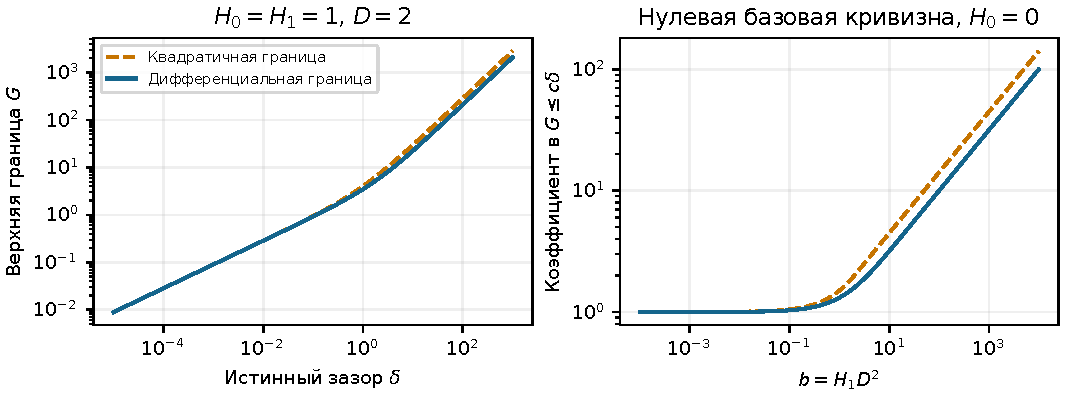
\includegraphics[width=\linewidth]{ru/figures/gap_geometry.pdf}
\caption{Поточечные теоретические границы. Дифференциальная огибающая
сохраняет изменение значения функции вдоль отрезка; сравнение с
фиксированной квадратичной моделью дано в~\eqref{eq:sharpbridge}.
При нулевой базовой кривизне точный линейный коэффициент равен
$\sqrt b\coth\sqrt b$. Это неравенства для класса функций,
а не траектории оптимизации или измерения времени.}
\label{fig:geometry}
\end{figure}

\begin{theorem}[Геометрическая сертификатная оценка AFW]\label{thm:geometric}
Предположим $H_0+H_1>0$ и~\eqref{eq:geometry}. Положим
\[
 J_*=\ceil{\log_2(U_0/\eta_\varepsilon)},\qquad
 P_*=\ceil{\log_2\max\{1,M/[2(H_0+H_1U_0)]\}}.
\]
При $0<\varepsilon<U_0$ тот же алгоритм достигает
$U_N\le\varepsilon$ за
\begin{equation}\label{eq:geometriccount}
 N\le2\ceil{P_*+(6+4H_0D^2/\kappa)J_*+8H_1D^2U_0/\kappa}
       +|S_0|-1
\end{equation}
обновлений. Формула~\eqref{eq:functioncount} остаётся верной.
Ни $H_0,H_1,\kappa$, ни $f_Q^*$ не являются входами алгоритма.
\end{theorem}
\begin{proof}
Анализируем фазы истинной ошибки $b_j/2<\delta_k\le b_j$ с
$b_j=U_0/2^j$ до достижения $\delta\le\eta_\varepsilon$.
Их положительные границы $C_j=2(H_0+H_1b_j)$ убывают не более
чем вдвое. Начальная истинная ошибка может пропустить фазы;
лемма~\ref{lem:lag} всё равно ограничивает запаздывающие обновления
числом $P_*+J_*$. На контролируемом хорошем шаге
\[
 f_k-f_{k+1}\ge\delta_k\min\{1/2,\kappa/(C_jD^2)\}
 >\min\{b_j/4,\kappa b_j/(2C_jD^2)\}.
\]
Для полного FW-шага используем $g\ge G\ge\delta$; для
необрезанного шага — условие~\eqref{eq:geometry}.
Бюджет фазы $b_j$ допускает не более
$5+4H_0D^2/\kappa+4H_1D^2b_j/\kappa$ контролируемых хороших
обновлений. Суммируем $\sum_{j<J_*}b_j<2U_0$, добавляем
запаздывающие обновления и применяем~\eqref{eq:dropcount}.
Теорема~\ref{lem:bridge} гарантирует, что к этому моменту фактический
сертификат уже прошёл порог.
\end{proof}

Для фиксированных задачи и инициализации зависимость от точности
логарифмическая. Явная фазовая цена $H_1$ пропорциональна $U_0$;
кроме того, $H_1$ входит в $J_*$ через~\eqref{eq:threshold}.
При выполнении геометрической гипотезы применимы обе AFW-оценки;
начальный вклад $U_0/\kappa$ означает, что геометрическая оценка
не всегда точнее выпуклой. Предполагать $H_0>0$ необязательно:
при $H_1>0$ границы положительны на положительных уровнях фаз.
Неаффинный пример — $f=t+(\max\{t,0\})^3$, $t=1/2-x$, на
$[-1/2,1/2]$ с $H_0=0,H_1=6$ и $\kappa=1/16$
(приложение~\ref{app:bridge}). На деле $H_0=0$ имеет более сильные
структурные следствия, доказанные далее без геометрического
неравенства~\eqref{eq:geometry}.

\section{Нулевая базовая кривизна: структура и конечная остановка}
\label{sec:zero}
Предельный случай $H_0=0$ качественно отличается от малого
положительного $H_0$. Утверждения ниже относятся к условному зазору
$\delta=f-f_Q^*$; условие кривизны выполняется на всём $Q$.

\begin{proposition}[Экспонированная оптимальная грань и общий градиент]
\label{prop:zeroface}
Пусть $H_0=0$. Для любого $x^*\in X^*:=\arg\min_Q f$ положим
$g^*=\nabla f(x^*)$. Тогда
\begin{equation}\label{eq:zeroface}
 X^*=\{x\in Q:\inner{g^*}{x-x^*}=0\}.
\end{equation}
Во всех оптимальных точках градиент равен одному и тому же $g^*$,
а для $x\in Q$
\begin{equation}\label{eq:zerograd}
 \norm{\nabla f(x)-g^*}\le\tfrac12H_1D\delta(x).
\end{equation}
В частности, стационарный в объемлющем пространстве оптимум $g^*=0$
вынуждает $f$ быть постоянной на $Q$. Непостоянная функция этого
класса с нулевой базовой кривизной также не может иметь оптимум в
относительной внутренности.
\end{proposition}
\begin{proof}
Оптимальность и выпуклость дают $w:=\inner{g^*}{x-x^*}\ge0$ и
$\delta(x)\ge w$. Для $h(t)=\delta(x^*+t(x-x^*))$ условие
кривизны даёт $h''\le H_1\norm{x-x^*}^2h$, причём $h(0)=0$ и
$h'(0)=w$. То же сравнение с положительным ядром, что и в
теореме~\ref{lem:bridge}, даёт
\[
 0\le h(t)\le w\frac{\sinh(rt)}r,\qquad
 r=\sqrt{H_1}\norm{x-x^*},
\]
где при $r=0$ отношение равно $t$. Поэтому $w=0$ влечёт
$h(1)=0$, что доказывает~\eqref{eq:zeroface}.
Отрезок между двумя оптимумами лежит в $X^*$; гессиан на нём
нулевой по предполагаемому ограничению нормы, поэтому интегрирование
показывает совпадение градиентов. На отрезке от $x^*$ до $x$
выпуклость даёт $h(t)\le t\delta(x)$. Интегрируя норму гессиана,
получаем
\[
 \norm{\nabla f(x)-g^*}
 \le H_1\norm{x-x^*}\int_0^1h(t)\,dt
 \le\tfrac12H_1D\delta(x).
\]
В оптимуме из относительной внутренности линейный функционал $g^*$
постоянен на аффинной оболочке $Q$, поэтому~\eqref{eq:zeroface}
даёт $X^*=Q$.
\end{proof}

Пусть теперь $Q=\operatorname{conv}(\mathcal A)$ — многогранник
с конечным множеством атомов, а $f$ непостоянна на $Q$.
Обозначим $\mathcal A_*:=\mathcal A\cap X^*$ и
\begin{equation}\label{eq:atommargin}
 m:=\min_{v\in\mathcal A\setminus\mathcal A_*}
              \inner{g^*}{v-x^*}>0.
\end{equation}
Для любого активного представления $x=\sum\lambda_vv$ масса вне
оптимальной грани удовлетворяет
\begin{equation}\label{eq:badmass}
 \theta:=\sum_{v\notin\mathcal A_*}\lambda_v
 \le\frac{\inner{g^*}{x-x^*}}m\le\frac{\delta(x)}m.
\end{equation}
Замена неоптимальных атомов любой точкой $X^*$ показывает, что
$\operatorname{dist}(x,X^*)\le D\theta$. Следовательно, сама
модель влечёт глобальную оценку слабой остроты
\[
 \delta(x)\ge(m/D)\operatorname{dist}(x,X^*).
\]
Независимая гипотеза квадратичного роста здесь не нужна.
Конечность множества атомов существенна: для аффинной функции
$f(x)=1-x_1$ на единичном диске
\[
\delta(\cos t,\sin t)/\operatorname{dist}((\cos t,\sin t),X^*)
=|\sin(t/2)|\to0.
\]
Таким образом, нулевая базовая кривизна на
произвольном компактном выпуклом множестве не влечёт слабой остроты.

\begin{theorem}[Конечная точная остановка AFW с обратным поиском]
\label{thm:zerofinite}
Пусть $H_0=0$, множество атомов конечно и $U_0>0$. Положим
\[
 b=H_1D^2,\quad
 c_b=\begin{cases}\sqrt b\coth\sqrt b,&b>0,\\1,&b=0,\end{cases}
 \qquad \overline L=\max\{M,2H_1U_0\},
\]
\begin{equation}\label{eq:zerothreshold}
 \tau=\min\left\{\frac{U_0}2,
       \frac{m}{4(1+b+c_b)}\right\},\qquad
 J_0=\ceil{\log_2(U_0/\tau)}.
\end{equation}
Определим два потенциала инициализации:
\[
 P=\ceil{\log_2\max\{1,MD^2/U_0\}},\qquad
 Q_0=\ceil{\log_2\max\{1,8\overline L D^2\tau/m^2\}}.
\]
Стандартный алгоритм AFW с обратным поиском, продолжаемый с нулевым
допуском остановки, достигает точного оптимума и $U_N=0$ за
\begin{equation}\label{eq:zerofinite}
 N\le2\big[P+\ceil{(6+16b)J_0}+Q_0\big]+|S_0|-1
\end{equation}
обновлений. После первой исходной точки с $U\le\tau$ каждое
неоптимальное обновление выбирает направление удаления; до момента,
когда остаются лишь максимальные удаления неоптимальных атомов,
происходит не более $Q_0$ дополнительных хороших обновлений.
Числа градиентов и полных LMO равны $N+1$, а
\[
 N_f\le1+2N+\ceil{\log_2\max\{1,2H_1U_0/M\}}.
\]
Ни $m,H_1,f_Q^*$, ни порог $\tau$ не являются входами алгоритма.
Не требуется ни гипотеза~\eqref{eq:geometry}, ни положительная
константа сильной выпуклости. Утверждения предполагают точную арифметику.
\end{theorem}
\begin{proof}
Огибающая принятой кривизны даёт $L_k\le\overline L$ для всех
обновлений. Рассмотрим неоптимальную исходную точку с $U\le\tau$;
тогда $0<\delta\le\tau$. По~\eqref{eq:zerograd} различие между
текущей и оптимальной разностями градиентных оценок любых двух атомов
не превосходит $b\delta/2$. Поэтому текущая оценка любого
неоптимального атома строго больше оценки любого оптимального.
LMO возвращает оптимальный атом. У неоптимальной исходной точки
есть активный неоптимальный атом, и максимизатор удаления $v$
обязательно неоптимален. Его зазор удовлетворяет
\[
 g_{\mathrm A}=\inner{\nabla f(x)}{v-x}
 \ge m-\delta-b\delta/2\ge3m/4.
\]
В то же время теорема~\ref{lem:bridge} даёт
$G\le c_b\delta\le m/4$. Поэтому алгоритм выбирает удаление.
Вес этого атома не превосходит $\theta\le\delta/m<1/2$, откуда
\[
 \alpha_{\max}\le2\delta/m.
\]
Положим $R=m^2/(8D^2\tau)$. Поскольку
\[
 2H_1\tau/R=16b\tau^2/m^2
 \le b/(1+b+c_b)^2\le1,
\]
принятая оценка выше $R$ обязательно получена делением пополам на
первой пробе; приёмка после отказа даёт менее
$2H_1\delta\le R$. При входе унаследованная оценка не превосходит
$\overline L$, поэтому таких делений не более $Q_0$.
Принятая оценка не выше $R$ остаётся не выше $R$ по локальной
огибающей и удовлетворяет
\[
 L_k\norm d^2\alpha_{\max}
 \le 2RD^2\delta/m\le m/4<g_{\mathrm A}.
\]
Каждая такая проба обрезается на допустимой верхней границе и удаляет
неоптимальный атом. Целевая функция и $U$ убывают, поэтому локальные
условия сохраняются. После конечного числа удалений все активные
атомы оптимальны. Тогда $G=0$, и оплаченная финальная проверка даёт
$U=0$.

Для подсчёта предшествующих обновлений применим фазовое доказательство
теоремы~\ref{thm:afw} до первой исходной точки с $U\le\tau$.
Оно ограничивает суммарное число хороших обновлений до этой точки
величиной $P+\ceil{(6+16b)J_0}$. Локальный аргумент допускает
не более $Q_0$ дополнительных хороших обновлений. Глобальный подсчёт
удалений~\eqref{eq:dropcount} доказывает~\eqref{eq:zerofinite}.
Тождество числа вызовов функции и огибающая дают заявленную
оракульную оценку, включая отказы.
\end{proof}
Здесь $J_0$ не зависит от $M$. Поэтому для фиксированных функции
и старта большое $M$ даёт лишь $O(\log M)$ через $P,Q_0$, без
дополнительного множителя $H_1D^2$ при этой цене инициализации.

Конечная идентификация активного множества при строгой
дополняемости — известная теория~\cite[теорема 3.1 и приложение]{bomze},
а не новое общее явление. Garber~\cite[теоремы 4--5]{garber} также
даёт результаты конечной сходимости и идентификации грани для
вариантов FW с линейным поиском. Здесь сама модель с нулевой базовой
кривизной вынуждает экспонированную грань совпадать со всем множеством
решений; идентификация этой грани точно решает задачу. Приведённые
порог и число проб специализируют механизм к унаследованной оценке
кривизны с делением и умножением на два, не требуя сходимости к
конкретному оптимуму. Приоритет перед всеми теоремами идентификации
не заявляется.

\paragraph{Почему предельный случай существенен.}
Вывод не переносится на произвольное $H_0>0$. На $[-1,1]$
возьмём $f(x)=h x^2/2$, $h>0$, $0<x_0<1$ и $M=3h$.
Обратный поиск на каждом обновлении принимает $L_k=3h/2$:
начальная первая проба принимается, а каждая последующая проба
$3h/4$ отклоняется для этого ненулевого квадратичного шага.
Выбранное направление — FW в обычном представлении через два
конца отрезка, и
\[
 x_{k+1}=x_k-f'(x_k)/(3h/2)=x_k/3.
\]
Поэтому ни одна конечная итерация не оптимальна, сколь бы мало ни
было $h=H_0>0$. Конечная идентификация оптимальной грани в общем
случае не решает непостоянную на этой грани целевую функцию.

\section{Эксперименты: инициализация, геометрия и остановка}
\label{sec:experiments}
Эксперименты проверяют поведение при конечном бюджете, а не точность
констант худшего случая. Все методы используют один скалярный
сертификат, кроме явно указанных вариантов контроля остановки.
Различаются бюджеты функции, градиента и полного LMO; произвольные
коэффициенты пересчёта и ранжирование по времени не вводятся.
Просмотры активного множества и оценки атомов AFW учитываются
отдельно. Запуски, достигшие лимита, остаются в сводках.

\subsection{Целевые функции счётных данных с проверенными границами кривизны}
Основные протоколы реальных данных используют Seoul Bike Sharing
Demand~\cite{seoul} и Metro Interstate Traffic Volume~\cite{metro};
сохранены неизменённые официальные файлы, хеши и атрибуция CC BY 4.0.
Устойчивая хронологическая сортировка и первые 80\% строк задают
обучающие данные. Признаки, кроме свободного члена, преобразуются как
$\tanh((v-\bar v_{\rm train})/s_{\rm train})$ с использованием
только обучающих статистик; свободный член включён и ограничен.
Повторные временные метки источника сохраняют исходные веса.
Оптимизируется обучающая функция, а не критерий качества прогноза.

При нормированном отклике $t_i=y_i/\bar y_{\rm train}$ и
$c_i=t_i\log t_i-t_i$ с соглашением $0\log0=0$ целевая функция равна
\begin{equation}\label{eq:poisson}
 f(x)=\frac1m\sum_i\{e^{a_i^\top x}-t_i a_i^\top x+c_i\}
          +\frac{\mu}{2}\norm x^2,\qquad \norm x_1\le R,
 \quad\mu=0.01.
\end{equation}
Квадратичная регуляризация применяется ко всем координатам, включая
свободный член. Поскольку $\norm{a_i}_\infty=1$ и
$\operatorname{mean}(t_i)=1$, корректные константы относительно
условного оптимума имеют вид
\begin{equation}\label{eq:poissonconstants}
 H_1=\max_i\norm{a_i}^2,\qquad H_0=\mu+H_1(1+R),\qquad
 L_Q=\mu+e^R\lambda_{\max}(A^\top A/m).
\end{equation}
Норма гессиана не превосходит
$\mu+H_1\operatorname{mean}(e^{a_i^\top x})$.
Так как $f_Q^*\le f(0)$, формула функции даёт
\[
 \operatorname{mean}(e^{a_i^\top x})\le\delta+1+R.
\]
Это аналитические верхние оценки, а не подогнанные или минимальные
константы. На компактной области существует и глобальная граница
Липшица.

\begin{table}[htbp]
\centering\small
\caption{Протоколы счётных данных. $R_*$ — $\ell_1$-норма автономного безусловного эталона; радиусы равны $R_*/2$ и $2R_*$. Ширины относятся к численным эталонным интервалам без направленного округления. На каждом радиусе используются все $2d$ знаковых координатных вершин.}
\label{tab:data}
\begin{tabular}{lrrrrr}
\toprule
Данные & Обучающих строк & $d$ & $R_*$ & $H_1$ & Макс. ширина \\
\midrule
Seoul & 7008 & 15 & 4.575821 & 8.897 & 4.2e-08 \\
Metro & 38563 & 12 & 1.431745 & 6.208 & 2.3e-09 \\
\bottomrule
\end{tabular}
\end{table}

Автономный эталон на основе метода Ньютона с демпфированием оценивает
$R_*=\norm{x^*_{\rm unc}}_1$. Радиусы $R_*/2$ и $2R_*$ дают
контроли с активным ограничением и внутренним оптимумом, с независимо
пересчитанными условными численными эталонами. Каждый эталон использует
допустимое значение как верхнюю границу и свою выпуклую касательную
нижнюю границу с LMO. Это численные интервалы без направленного
округления, а не формальные интервальные сертификаты. Они никогда не
подаются на вход решателям. После запуска ошибки оцениваются с этой
численной точностью. Все $2d$ знаковых координатных вершин используются
ровно один раз на каждом радиусе: всего 108 условий «набор данных /
радиус / старт». Радиусы и старты внутри одного набора используют
общие обучающие данные и не являются независимыми наборами.

\subsection{Общие бюджеты функции и неуспешные запуски}
Четыре стандартных BT-варианта сочетают FW/AFW с $M=1$ или
$U_0/D^2$. Два информированных контроля короткого шага используют
$L=H_0+H_1U_k$ с FW/AFW и обозначаются Q. Они получают константы
из~\eqref{eq:poissonconstants}; BT их не получает. Исходный архив
шести методов содержит 648 запусков. Мы добавляем 108 запусков AC-FW
на точно тех же условиях, сохраняя все прежние записи.

AC-FW — независимая реализация алгоритмов 1--2
из~\cite{autoconditioned} с формулой (6) и параметром $\delta=1$.
Обязательный начальный переход к вершине LMO и оба начальных вызова
функции и градиента оплачиваются. Отказ расходует внешнюю итерацию и
вызов функции, сохраняя старый градиент; полные LMO также учитываются.
Предположение источника о глобальной липшицевости градиента на $\R^d$
не выполняется для~\eqref{eq:poisson}, поэтому запуски на компакте —
эмпирическое сравнение, а не прямое применение глобальной теоремы.

Цель — $U\le10^{-5}$. BT/Q ограничены 1000 обновлениями; AC —
1000 внешними пробами, включая отказы. Основное сравнение использует
вместо этого не более 1000 вызовов функции: каждый незавершённый
запуск может достичь этого бюджета до своего лимита, а результаты
успешных запусков переносятся на последующие бюджеты. Каждый префикс —
последняя полностью оплаченная исходная точка в пределах бюджета,
восстановленная из полного журнала без интерполяции между прореженными
строками. При сравнении по одному оракулу остальные типы не ограничены.

\begin{table}[htbp]
\centering\small
\caption{Сертифицированные старты при общем бюджете 1000 вызовов функции. Каждый незавершённый запуск достигает бюджета до лимита; завершённые результаты переносятся вперёд. В каждой ячейке Seoul 30 стартов, Metro 24. $F/A$: FW/AFW; индексы $1,U$: начальные $M=1,U_0/D^2$; $Q$: короткий шаг с известной кривизной; AC: автоматически обусловленный FW с оплаченной предварительной обработкой.}
\label{tab:budget}
\begin{tabular}{llrrrrrrr}
\toprule
Данные & $R/R_*$ & $F_1$ & $F_U$ & $A_1$ & $A_U$ & $F_Q$ & $A_Q$ & AC \\
\midrule
Seoul & 0.5 & 0 & 0 & 30 & 30 & 0 & 0 & 0 \\
Seoul & 2 & 0 & 0 & 0 & 0 & 0 & 0 & 0 \\
Metro & 0.5 & 2 & 3 & 24 & 24 & 1 & 24 & 13 \\
Metro & 2 & 0 & 0 & 0 & 0 & 0 & 0 & 0 \\
\bottomrule
\end{tabular}
\end{table}

\begin{figure}[htbp]
\centering
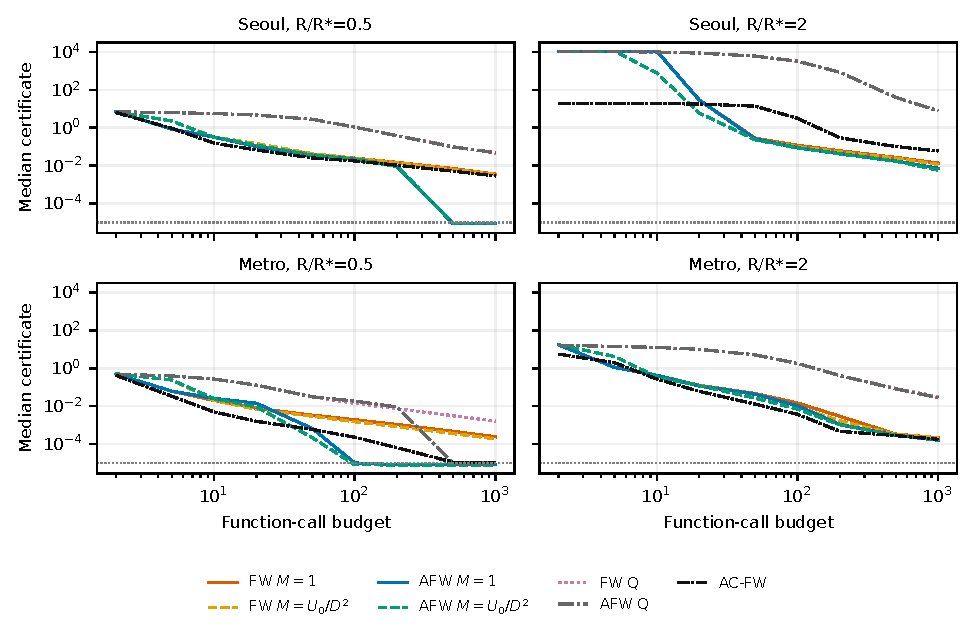
\includegraphics[width=\textwidth]{figures/count_comparators.pdf}
\caption{Медианы скалярных сертификатов по всем различным вершинам
при заданных бюджетах вызовов функции. Кривые включают неуспешные
запуски и оплаченную предварительную обработку AC-FW; завершённые
результаты переносятся вперёд. Горизонтальный пунктир — $10^{-5}$.
BT не получает кривизну, Q получает аналитические $H_0,H_1$.
Это парные конечные условия, а не доверительные полосы для
генеральной совокупности задач.}
\label{fig:counts}
\end{figure}

При активных радиусах обе инициализации AFW-BT сертифицируют каждый
старт за 1000 вызовов функции. FW-BT не сертифицирует ни одного
старта Seoul и лишь 2/24 или 3/24 на Metro. AC-FW даёт 13/24
успехов на активном Metro и ни одного на активном Seoul.
AFW-Q с известной кривизной успешен на всех активных стартах Metro,
но ни на одном активном Seoul, что иллюстрирует консервативность
аналитических параметров. При внутренних радиусах ни один метод
этого сравнения семи методов со скалярным сертификатом не достигает
цели за 1000 вызовов функции. Результаты к лимиту и медианы вызовов
с учётом цензурирования приведены отдельно в таблице~\ref{tab:counts}.

Эталоны отделяют оставшуюся ошибку от запаздывания остановки.
На внутреннем радиусе Metro у всех 24 стартов каждого BT-варианта
верхняя граница численной эталонной ошибки не больше $10^{-5}$
к исходному концу запуска, но у FW нет успехов по скалярному
сертификату, а у AFW лишь 6/24 или 7/24. На внутреннем Seoul
соответствующее условие эталонной ошибки выполняется у 12/30 и
18/30 AFW-стартов, хотя ни один скалярный BT-вариант не останавливается.
Следовательно, неуспех сертификата не равнозначен большой оставшейся
ошибке по функции.

\subsection{Контроль инициализации и единиц целевой функции}
Отдельное исследование $2\times2$ контролирует исходную точку против
обязательной вершины LMO и обновления AC против BT. Все четыре
условия оплачивают одинаковую обработку двух исходных точек,
сохраняют обе касательные границы и начинают первую пробу с одной
секущей кривизны. Лишь AC/вершина является исходным опубликованным
вариантом; остальные условия изолируют факторы. Исследование содержит
280 запусков на 70 прежних согласованных условиях и не вводит новых
наборов данных. Таблица~\ref{tab:init} показывает все три заданных
семейства с активным ограничением, включая неблагоприятное
масштабированное. Их конструкция и тождество запаса активной грани
даны в приложении~\ref{app:protocol}.

\begin{table}[htbp]
\centering\small
\caption{Контроль старта на трёх заданных семействах с активным ограничением, по десять согласованных экземпляров. Числа — сертифицированные старты за 1000 вызовов функции. O/V: исходная точка/обязательная начальная вершина LMO. Последний столбец — описательная парная медиана отношения сертификатов BT-V/AC-V и 95\%-й процентильный бутстреп-интервал, а не оценка ускорения.}
\label{tab:init}
\begin{tabular}{lrrrrl}
\toprule
Семейство & AC-O & AC-V & BT-O & BT-V & Отношение [интервал] \\
\midrule
active & 1 & 10 & 0 & 10 & 1.049 [0.935, 1.257] \\
active\_scaled & 0 & 0 & 0 & 0 & 1.530 [0.822, 1.750] \\
active\_highdim & 6 & 8 & 2 & 8 & 1.231 [0.798, 2.117] \\
\bottomrule
\end{tabular}
\end{table}

На семействе active смена старта повышает число успехов с 1 до 10
для AC и с 0 до 10 для BT. Описательный интервал отношения
сертификатов BT/AC при старте из вершины включает единицу.
Масштабированное семейство не решается ни одним из четырёх контролей.
Поэтому прежнее сравнение с вершинным стартом не изолирует преимущество
правила обновления.

Единицы целевой функции дают другой контроль. При
$\widetilde f=af+b$, $a>0$, умножение $M$ и $\varepsilon$ на $a$
сохраняет точные итераты, пробы и индекс остановки, поскольку
$G,U,L$ масштабируются вместе. Поэтому $M=U_0/D^2$ автоматически
эквивариантно; фиксация численного значения $M$ меняет эффективную
инициализацию. Отдельное исследование радиусов и масштабов на реальных
данных подтверждает счётчики во всех 60 парных сравнениях масштабов
для каждого метода с инициализацией по сертификату. Это элементарное
свойство не устанавливает более быстрый алгоритм.

\subsection{Причинные контроли остановки на фиксированных BT-траекториях}
Повторяются 432 исходные BT-траектории исследования счётных данных
с точным совпадением исходных концов и оракульных счётчиков.
Пять причинных мониторов дают 2160 зависимых профилей остановки.
Непересекающиеся блоки из $K=8,32,128$ оплаченных аффинных касательных
дают нижнюю оценку с одним дополнительным полным LMO на завершённый
блок; скалярная огибающая сохраняется. Отдельный стандартный контроль
получает $\mu=0.01$ и использует
$f-\norm{\nabla f}^2/(2\mu)$ как нижнюю оценку.
Приложение~\ref{app:monitors} доказывает корректность и раздельный
учёт оракулов; размеры блоков фиксируются до результатов, и ни один
монитор не читает эталон.

\begin{table}[htbp]
\centering\small
\caption{Раздельные причинные контроли на 432 точно повторённых BT-траекториях, дающие 2160 зависимых профилей. Используется первая остановка профиля или исходный лимит. Последний столбец сравнивает суммарные LMO направления и сертификата со скалярным профилем. Контроль с известным $\mu$ получает аналитический коэффициент регуляризации; блоки его не получают.}
\label{tab:monitors}
\begin{tabular}{lrrr}
\toprule
Профиль & Сертифицировано & Ранних префиксов & Больше LMO \\
\midrule
scalar & 129 & 0 & 0 \\
block\_8 & 129 & 0 & 432 \\
block\_32 & 129 & 0 & 425 \\
block\_128 & 129 & 0 & 380 \\
known\_mu & 226 & 110 & 0 \\
\bottomrule
\end{tabular}
\end{table}

Ни один проверенный блок не даёт более ранней остановки.
Контроль с известным $\mu$ даёт 226 успехов вместо 129 и 110 более
ранних префиксов, без дополнительных LMO, но с дополнительной
информацией о модели. На внутреннем Metro каждый BT-вариант теперь
достигает 24/24 успехов к исходному концу; оба AFW-варианта делают
это за 1000 вызовов функции. Внутренний Seoul остаётся трудным:
AFW даёт лишь 4/30 или 10/30 успехов к концу и ни одного за
1000 вызовов функции. Эти контроли не устанавливают адаптацию к
неизвестной сильной выпуклости и не оценивают точный двойственный
сертификат Фенхеля с усреднённым градиентом из~\cite{pedregosa}.
Они показывают, что наблюдаемая стоимость остановки — отдельный
практический вопрос.

\section{Обсуждение}
Фазовый аргумент заменяет единую глобальную границу кривизны
последовательностью границ на уровнях исходных точек, сохраняя LMO на
всём допустимом множестве. Результат — гарантия для накопленного
скалярного сертификата и учёт каждой отклонённой пробы функции.
Это различие существенно, когда малой ошибки по функции ещё
недостаточно, чтобы алгоритм мог удостоверить остановку. Как показывает
аффинный пример, слагаемое инициализации неотделимо от заданного
правила деления оценки пополам.

Эксперименты подтверждают необходимость контроля инициализации,
единиц целевой функции и активной геометрии. Универсального практического
ранжирования они не устанавливают. Положительное $H_1$ на компакте не
исключает глобальной константы Липшица, а аналитические константы могут
быть консервативными. Логарифмическая AFW-теорема при положительной
базовой кривизне требует дополнительного геометрического неравенства.
При нулевой базовой кривизне сама модель даёт экспонированную
оптимальную грань и конечную остановку; это граничный режим задачи
с ограничениями, а не общая модель непостоянной функции потерь с
достигнутым внутренним минимумом. Оценки в точной арифметике сами по
себе не обеспечивают надёжности при конечной точности; детерминированные
поправки оракулов в приложении~\ref{app:inexact} устанавливают лишь
корректность сертификата. Открытыми остаются расширения на направления
с контролируемым шумом, парные перестановки и адаптивный слайдинг с
учётом всех внутренних линейных оракулов.
\begin{otherlanguage}{english}
\begin{thebibliography}{99}
\bibitem{braun} G.~Braun, A.~Carderera, C.~W.~Combettes, H.~Hassani,
A.~Karbasi, A.~Mokhtari, and S.~Pokutta. Conditional Gradient Methods.
\href{https://arxiv.org/abs/2211.14103v5}{arXiv:2211.14103v5}, 2025.
\bibitem{pedregosa} F.~Pedregosa, G.~Negiar, A.~Askari, and M.~Jaggi.
Linearly Convergent Frank-Wolfe with Backtracking Line-Search.
\emph{AISTATS}, 2020. \href{https://arxiv.org/abs/1806.05123}{arXiv:1806.05123}.
\bibitem{lacostejaggi} S.~Lacoste-Julien and M.~Jaggi.
On the Global Linear Convergence of Frank-Wolfe Optimization Variants.
\emph{NeurIPS}, 2015.
\href{https://arxiv.org/abs/1511.05932}{arXiv:1511.05932}.
\bibitem{warmup} F.~Alimisis, R.~Islamov, and A.~Lucchi.
Why Do We Need Warm-up? A Theoretical Perspective.
\href{https://arxiv.org/abs/2510.03164v2}{arXiv:2510.03164v2}, 2026.
\bibitem{kale} S.~Kale, J.~D.~Lee, C.~De~Sa, A.~Sekhari, and K.~Sridharan.
From Gradient Flow on Population Loss to Learning with Stochastic Gradient Descent.
\href{https://arxiv.org/abs/2210.06705v1}{arXiv:2210.06705v1}, 2022.
\bibitem{caoselfbound} D.~Y.~Cao, A.~Y.~Chen, K.~Sridharan, and B.~Tang.
Efficiently Escaping Saddle Points under Generalized Smoothness via Self-Bounding Regularity.
\href{https://arxiv.org/abs/2503.04712v3}{arXiv:2503.04712v3}, 2026.
\bibitem{bomze} I.~M.~Bomze, F.~Rinaldi, and D.~Zeffiro.
Active set complexity of the Away-step Frank-Wolfe Algorithm.
\href{https://arxiv.org/abs/1912.11492}{arXiv:1912.11492}, 2019.
\bibitem{garber} D.~Garber.
Revisiting Frank-Wolfe for Polytopes: Strict Complementarity and Sparsity.
\href{https://arxiv.org/abs/2006.00558}{arXiv:2006.00558}, 2020.
\bibitem{lobanovkoloskova} A.~Lobanov and A.~Koloskova.
Avoiding Bias in Clipped SGD for Overparameterized Models under Generalized Smoothness.
\href{https://arxiv.org/abs/2605.14800v2}{arXiv:2605.14800v2}, 2026.
\bibitem{lobanov} A.~Lobanov.
A Few Accelerated Algorithms for Convex Optimization under $(H_0,H_1)$-Smoothness.
\href{https://arxiv.org/abs/2608.04884}{arXiv:2608.04884}, 2026.
\bibitem{vyguzov} A.~A.~Vyguzov and F.~S.~Stonyakin.
Frank-Wolfe Algorithms for $(L_0,L_1)$-smooth functions.
\href{https://arxiv.org/abs/2510.16468v5}{arXiv:2510.16468v5}, 2026.
\bibitem{selfconcordant} P.~Dvurechensky, K.~Safin, S.~Shtern, and M.~Staudigl.
Generalized Self-Concordant Analysis of Frank-Wolfe Algorithms.
\href{https://arxiv.org/abs/2010.01009}{arXiv:2010.01009}, 2020.
\bibitem{bregmanfw} S.~Takahashi, S.~Pokutta, and A.~Takeda.
Fast Frank--Wolfe Algorithms with Adaptive Bregman Step-Size for Weakly Convex Functions.
\emph{ICLR}, 2026.
\href{https://arxiv.org/abs/2504.04330v4}{arXiv:2504.04330v4}.
\bibitem{adcgs} S.~Takahashi.
Adaptive Conditional Gradient Sliding: Projection-Free and Line-Search-Free Acceleration.
\href{https://arxiv.org/abs/2601.20443v2}{arXiv:2601.20443v2}, 2026.
\bibitem{wirth} E.~Wirth, J.~Pe\~na, and S.~Pokutta.
Fast convergence of Frank-Wolfe algorithms on polytopes.
\href{https://arxiv.org/abs/2406.18789v3}{arXiv:2406.18789v3}, 2025.
\bibitem{restartfw} T.~Kerdreux, A.~d'Aspremont, and S.~Pokutta.
Restarting Frank-Wolfe: Faster Rates under H\"olderian Error Bounds.
\href{https://arxiv.org/abs/1810.02429v4}{arXiv:1810.02429v4}, 2021.
\bibitem{zhao} R.~Zhao.
New Analysis of an Away-Step Frank-Wolfe Method for Minimizing
Logarithmically-Homogeneous Barriers.
\href{https://arxiv.org/html/2305.17808v4}{arXiv:2305.17808v4}, 2023.
\bibitem{autoconditioned} K.-H.~Giang-Tran, S.~Shafiee, and N.~Ho-Nguyen.
Auto-Conditioned Frank-Wolfe Algorithms.
\href{https://arxiv.org/abs/2605.15512}{arXiv:2605.15512}, 2026.
\bibitem{khademi} A.~Khademi and A.~Silveti-Falls.
Adaptive Conditional Gradient Descent.
\href{https://arxiv.org/abs/2510.11440v1}{arXiv:2510.11440v1}, 2025.
\bibitem{yagishita} S.~Yagishita and M.~Ito.
Simple linesearch-free first-order methods for nonconvex optimization.
\href{https://arxiv.org/abs/2509.14670}{arXiv:2509.14670}, 2025.
\bibitem{lacoste2016} S.~Lacoste-Julien.
Convergence Rate of Frank-Wolfe for Non-Convex Objectives.
\href{https://arxiv.org/abs/1607.00345}{arXiv:1607.00345}, 2016.
\bibitem{seoul} Seoul Bike Sharing Demand [Dataset].
UCI Machine Learning Repository, 2020.
\href{https://doi.org/10.24432/C5F62R}{doi:10.24432/C5F62R}. CC BY 4.0.
\bibitem{metro} J.~Hogue. Metro Interstate Traffic Volume [Dataset].
UCI Machine Learning Repository, 2019.
\href{https://doi.org/10.24432/C5X60B}{doi:10.24432/C5X60B}. CC BY 4.0.
\bibitem{karimi} H.~Karimi, J.~Nutini, and M.~Schmidt.
Linear Convergence of Gradient and Proximal-Gradient Methods Under the
Polyak--{\L}ojasiewicz Condition.
\href{https://arxiv.org/abs/1608.04636v4}{arXiv:1608.04636v4}, 2020.
\bibitem{wdbc} W.~Wolberg, O.~Mangasarian, N.~Street, and W.~Street.
Breast Cancer Wisconsin (Diagnostic) [Dataset]. UCI Machine Learning Repository, 1993.
\href{https://doi.org/10.24432/C5DW2B}{doi:10.24432/C5DW2B}.
\bibitem{bike} H.~Fanaee-T. Bike Sharing [Dataset]. UCI Machine Learning Repository, 2013.
\href{https://doi.org/10.24432/C5W894}{doi:10.24432/C5W894}. CC BY 4.0.
\end{thebibliography}

\end{otherlanguage}
\appendix
\section{Шаги сравнения и нормировка сертификата}
\label{app:explicit}
Если заданы $H_0,H_1$, рассмотрим
\[
 \alpha=\min\{1,G/[(H_0+H_1U)q^2]\},
\]
с полным шагом при нулевой кривизне. Аргумент спуска из
леммы~\ref{lem:local}, с учётом $U\ge\delta$, даёт
\[
 f_k-f_{k+1}\ge\frac12\min\{U_k,U_k^2/[D^2(H_0+H_1U_k)]\}.
\]
В фазе $b/2<U\le b$ продвижение не меньше
$\min\{b/4,b^2/(8D^2H_0+4D^2H_1b)\}$, поскольку правая часть
возрастает по $U>0$. Поэтому бюджет фазы допускает не более
$5+4H_1D^2+8H_0D^2/b$ обновлений. Суммирование по тем же
двоичным уровням доказывает
\begin{equation}\label{eq:explicitcount}
 N\le\ceil{(5+4H_1D^2)J+16H_0D^2/\varepsilon}.
\end{equation}
Для этого явного шага требуется $N+1$ вызовов каждого оракула.
Точная минимизация на отрезке даёт не меньшее продвижение, чем шаг
сравнения, поэтому наследует~\eqref{eq:explicitcount} без получения
$H_0,H_1$. Это не ограничивает внутренние вызовы функции или
градиента, необходимые для точного скалярного минимума. В расширенном
техническом отчёте также выведен гиперболический шаг того же порядка;
его элементарная функция не нужна для теоремы~\ref{thm:fw}.

Для полноты рассмотрим обратный поиск с нормировкой по сертификату:
он начинает с $\theta_{-1}=1$, пробует $\theta_{k-1}/2$, задаёт
$L=\theta U_k/D^2$ и удваивает $\theta$ при отказе квадратичной
проверки. Достаточный порог $T_k=D^2(H_0/U_k+H_1)$ не убывает.
Индукцией получаем
\[
 \theta_k\le\max\{2^{-k-1},2T_k\},\qquad
 L_k\le\max\{U_k/(2^{k+1}D^2),2(H_0+H_1U_k)\}.
\]
Действительно, приёмка первой пробы делит предыдущую границу пополам,
а после отказа принятая оценка меньше $2T_k$.
Значит, $L_k\le2H_0+(2H_1+1/(2D^2))U_k$. Применяя предыдущий
фазовый аргумент с этими эффективными константами, получаем
\[
 N\le\ceil{(7+8H_1D^2)J+32H_0D^2/\varepsilon}.
\]
Рекурсия $\theta_k=2^{r_k-1}\theta_{k-1}$ даёт
\[
 N_f\le1+2N+\ceil{\log_2\max\{1,2D^2(H_0/\varepsilon+H_1)\}}.
\]
В последней исходной точке перед обновлением $U>\varepsilon$,
что ограничивает $\theta_{N-1}$. Эта нормировка требует $D$ и
необязательна для двухфазного порядка. Теоремы~\ref{thm:fw}
и~\ref{thm:afw} относятся к обычному обратному поиску, а не к этому
отдельному варианту.

\section{Геометрические следствия и достигающие примеры}
\label{app:geometry}
Пусть $p=\inner{\nabla f(x)}{v-s}$ — парный зазор по полному
множеству атомов и текущему активному множеству. Выбранный зазор
FW/удаления не меньше $p/2$. Стандартное неравенство масштабирования
многогранника даёт для любого оптимального $x^*\ne x$
\[
 p\ge W\frac{\inner{\nabla f(x)}{x-x^*}}{\norm{x-x^*}}.
\]
См.~\cite[теорема 3]{lacostejaggi} и
\cite[леммы 3.4 и 3.6]{restartfw}. При квадратичном росте выберем
ближайший оптимум. Выпуклость и неравенство роста дают
$p\ge W\delta/\operatorname{dist}(x,X^*)
\ge W\sqrt{\gamma\delta/2}$. Поэтому
$g^2\ge\gamma W^2\delta/8$ и $\kappa=\gamma W^2/16$.
Монотонные итераты остаются в начальном множестве подуровня, где
предполагается рост. Единственность не требуется. При сильной
выпуклости
$\inner{\nabla f(x)}{x-x^*}\ge\delta+\mu\norm{x-x^*}^2/2$;
минимизация $\delta/r+\mu r/2$ по $r>0$ даёт
$p\ge W\sqrt{2\mu\delta}$ и $\kappa=\mu W^2/4$.
Эти геометрические следствия известны ранее.

\subsection{Равенство в огибающей зазора и нулевая базовая кривизна}
\label{app:bridge}
\paragraph{Квадратичное сравнение.}
При $C=D^2(H_0+H_1\delta)$ допустимый шаг
$t=\min\{1,G/C\}$ и лемма~\ref{lem:local} дают
$\delta\ge G^2/(2C)$ при $G\le C$ и
$\delta\ge G-C/2$ иначе. При $C=0$ используется полный шаг.
Обращение этого известного неравенства спуска даёт
\begin{equation}\label{eq:sharpbridge}
 G\le\widehat B(\delta):=
 \begin{cases}\sqrt{2C\delta},&2\delta\le C,\\
 \delta+C/2,&2\delta>C.\end{cases}
\end{equation}
Теорема~\ref{lem:bridge} сохраняет изменение кривизны вдоль отрезка
и усиливает это сравнение при $H_1>0$.

\paragraph{Достижимость при $H_1=0$.}
Пусть $Q=[-D/2,D/2]$, $x=D/2$ и $f(y)=h(y-z)^2/2$, $h>0$.
Для $z\in Q$ имеем $\delta=h(x-z)^2/2$ и
$G=hD(x-z)=\sqrt{2hD^2\delta}$, что достигает корневой ветви
\eqref{eq:sharpbridge} при $H_0=h,H_1=0$.
Для $z<-D/2$ условный оптимум равен $-D/2$,
$\delta=-hDz$ и $G=\delta+hD^2/2$, что достигает ветви полного
шага. Эти примеры также достигают предела точной огибающей при $H_1=0$.

\paragraph{Достижимость при $H_1>0$.}
Обозначим $k=\sqrt{H_1}$, $a=kD$, $c=H_0/H_1$ и возьмём
$Q=[0,D]$ с исходной точкой $x=0$. При $c>0$ и
$0<\delta\le c(\cosh a-1)$ положим
\[
 r=k^{-1}\operatorname{arcosh}(1+\delta/c),\qquad
 f(u)=c\big(\cosh(k(u-r))-1\big).
\]
Функция глобально выпукла, $f_Q^*=f(r)=0$, $f(0)=\delta$,
$f''=H_0+H_1f$, а градиент в исходной точке отрицателен.
Поэтому FW-атом равен $D$ и
$G=-Df'(0)=D\sqrt{2H_0\delta+H_1\delta^2}$.

При $\delta>c(\cosh a-1)$, включая все $\delta>0$ при $c=0$,
обозначим $E=E(\delta)$ и для $u\le D$ положим
\[
 f(u)=(\delta+c)\cosh(ku)-\frac{E}{a}\sinh(ku)-c.
\]
На $[0,D]$ выполняются $f(D)=0$ и
\[
 f'(D)=k\frac{c\cosh a-(\delta+c)}{\sinh a}<0.
\]
Тождество $f''=H_0+H_1f$ и эта производная в конце показывают,
что $f$ убывает и неотрицательна на отрезке: явно,
$f(u)+c=c\cosh(k(D-u))-[f'(D)/k]\sinh(k(D-u))$ при $u\le D$.
Она выпукла на всей левой полуоси. Для $u>D$ продолжим её как
\[
 f(u)=f'(D)(u-D)+\tfrac12H_0(u-D)^2.
\]
В точке $D$ совпадают значение, производная и вторая производная
обеих частей, поэтому продолжение глобально выпукло и принадлежит
$C^2$. Его условный оптимум равен $D$, $f(0)=\delta$ и
$G=-Df'(0)=E$. При $H_0=0$ получаем
$f(u)=\delta\sinh(k(D-u))/\sinh a$ для $u\le D$ с аффинным
продолжением за $D$. Эти конструкции доказывают оптимальность для
каждого набора параметров, а не только для фиксированной квадратичной
модели. Поскольку~\eqref{eq:sharpbridge} применимо к каждой
достигающей функции, они также доказывают
$E(\delta)\le\widehat B(\delta)$: новый порог никогда не меньше
квадратичного.

\paragraph{Точное глобальное следствие самоограничения.}
При другом предположении, когда условие гессиана выполняется на всём
$\R^d$ относительно конечного глобального инфимума $f^*$, имеем
\begin{equation}\label{eq:globalselfbound}
 \norm{\nabla f(x)}^2\le2H_0(f(x)-f^*)+H_1(f(x)-f^*)^2.
\end{equation}
Действительно, применим сравнение с положительным ядром на всём луче
$x-t\nabla f(x)/\norm{\nabla f(x)}$, $t>0$.
Неотрицательность $f-f^*$ ограничивает начальную направленную
производную величиной
\[
 \sqrt{H_1}\inf_{t>0}
 \frac{(f(x)-f^*+H_0/H_1)\cosh(\sqrt{H_1}t)-H_0/H_1}
 {\sinh(\sqrt{H_1}t)}
 =\sqrt{2H_0(f(x)-f^*)+H_1(f(x)-f^*)^2}.
\]
При $H_1=0$ используется квадратичный предел, а при $H_0=0<H_1$
— предел $t\to\infty$. Оценка достигается приведённой выше
глобальной cosh-функцией при $H_0,H_1>0$, квадратичной функцией
при $H_1=0<H_0$ и функцией $f(x)=A\exp(\sqrt{H_1}x)$,
$A>0$, при $H_0=0<H_1$; в последнем случае инфимум не достигается.
Это даёт точные константы глобальной модели.
Оценка~\cite[приложение G, лемма 6]{warmup} имеет большие
коэффициенты $9H_0/4$ и $27H_1/4$; точность там не заявляется.
Для аффинного ограничения второго порядка
\cite[следствие 1]{caoselfbound} вместо этого даёт
$\norm{\nabla f}^2\le2(H_0+H_1\delta)^2
\log(1+H_1\delta/H_0)/H_1$ при $H_0,H_1>0$.
Точное полиномиальное выражение~\eqref{eq:globalselfbound} устраняет
эту логарифмическую добавку. Сам принцип самоограничения известен
ранее~\cite[лемма 11]{kale}; здесь сравниваются лишь приведённые
константы и экстремизаторы. Одна лишь условная модель не
влечёт~\eqref{eq:globalselfbound}: непостоянная аффинная функция на
компактном отрезке имеет $H_0=H_1=0$ и ненулевой градиент.

\paragraph{Полиномиальный пример с нулевой базовой кривизной.}
Глобально выпуклый $C^2$-пример $f(x)=t+(\max\{t,0\})^3$,
$t=1/2-x\in[0,1]$ на $Q$, удовлетворяет
$f''(x)=6t\le6f(x)$, поэтому $H_0=0,H_1=6$.
Он не является сильно выпуклым. В неоптимальной внутренней точке
оба конца-атома активны, и выбранный зазор равен
$(1+3t^2)\max\{t,1-t\}\ge1/2$; неоптимальный конец также
удовлетворяет этому неравенству. Поскольку $\delta\le2$,
условие~\eqref{eq:geometry} выполнено с $\kappa=1/16$.
При нулевой ошибке геометрическое неравенство очевидно.
Это показывает невакуумность расширения на $H_0=0$.

\section{Контроли нижних границ и детерминированные ошибки оракулов}
\label{app:monitors}
Обозначим $g_j=\nabla f(x_j)$ и $a_j=f(x_j)-\inner{g_j}{x_j}$.
Для завершённого блока $B$ из $K$ последовательных оплаченных
исходных точек
\[
 b_B=\bar a_B+\min_{v\in Q}\inner{\bar g_B}v\le f_Q^*.
\]
Выпуклость даёт $f(v)\ge a_j+\inner{g_j}v$ для каждой точки;
усреднение и минимизация доказывают корректность.
Непересекающиеся блоки начинаются с исходной точки ноль;
незавершённый блок не вызывает оракул. Новая нижняя граница —
максимум $\ell_k$ и всех завершённых $b_B$.
На том же монотонном пути её сертификат не возрастает и не больше
$U_k$, поэтому первое пересечение порога происходит не позже по
обновлениям и вызовам функции или градиента. В исходной точке $k$
выполнено ровно $\lfloor(k+1)/K\rfloor$ дополнительных полных LMO.
Суммарная стоимость LMO не обязана уменьшаться. Мониторы не влияют
ни на линейный поиск, ни на начальное $M$; каждая указанная стоимость
относится к одному отдельному монитору без остальных диагностических
мониторов. Доступная по бюджету исходная точка оплачивает всю
запланированную проверку.

Эти равномерные блочные границы отличаются от двойственной величины
Фенхеля с усреднённым градиентом из~\cite[теорема 3]{pedregosa}.
Когда существует глобальная сопряжённая функция, равенство Фенхеля
и неравенство Йенсена дают
\[
 b_B=-\overline{f^*(g_j)}-\sigma_Q(-\bar g_B)
     \le-f^*(\bar g_B)-\sigma_Q(-\bar g_B).
\]
Здесь $f^*$ обозначает сопряжённую функцию, а не скалярный оптимум
$f_Q^*$. Перенос теоремы или весов усреднения той работы не
заявляется. При заданной корректной константе сильной выпуклости
$\mu$ оценка $f(x_j)-\norm{g_j}^2/(2\mu)\le f_Q^*$ следует из
минимизации квадратичной нижней модели на $\R^d$~\cite[приложение B]{karimi}.
Сохранение этих границ не требует LMO, но использует дополнительную
информацию. Нативные проверки остановки на одном синтетическом
внутреннем экземпляре проверяют все 20 пар «метод/профиль» по
конструкции достижимого префикса и инструментируют фактические
вызовы оракулов. Это не 2160 дополнительных нативных запусков решателя.

\subsection{Корректность сертификата при ограниченных детерминированных ошибках}
\label{app:inexact}
Если $|\widehat f-f(x)|\le\nu$,
$\norm{\widehat g-\nabla f(x)}\le\rho$ и
$\inner{\widehat g}s\le\min_{v\in Q}\inner{\widehat g}v+\eta$
с известными границами, то
\[
 \ell^{\rm safe}=\widehat f+\inner{\widehat g}{s-x}
                      -\nu-\rho D-\eta\le f_Q^*.
\]
Для каждого $v\in Q$ выпуклость даёт
$f(v)\ge\widehat f-\nu+\inner{\widehat g}{v-x}-\rho D
\ge\ell^{\rm safe}$; минимизируем по $v$.
Максимум таких нижних границ остаётся корректным, а
$\widehat f+\nu-\max_j\ell_j^{\rm safe}$ является верхним
сертификатом. Это утверждение о корректности, а не теорема сходимости
для шумных направлений. Эмпирическая дисперсия не является
детерминированной границей нормы.

\section{Дополнительные подробности протокола и контроли}
\label{app:protocol}
\paragraph{Признаки.}
Seoul использует восемь численных погодных признаков: температуру,
влажность, скорость ветра, видимость, точку росы, солнечную радиацию,
дождь и снег; синус/косинус часа и дня недели; индикаторы праздника
и функционирования. Metro использует температуру, дождь, снег,
облачность, синус/косинус часа, дня недели и дня года с периодом
365.25, а также индикатор праздника. Остальные текстовые категории
опущены. Постоянные на обучении признаки удаляются до преобразования
$\tanh$; кодировки источников и имена признаков записаны в манифестах.
Эти детерминированные решения принимаются до сравнения решателей.

\paragraph{Исходный вариант сравнения.}
Для $x\ne y$ оценка AC-FW равна
\[
 \ell(x,y)=\frac{2|f(y)-f(x)-\inner{\nabla f(x)}{y-x}|}{\norm{y-x}^2},
\]
а при $x=y$ — нулю. При обновлении берётся максимум этой пробной
оценки и $r_kL_k$, где $r_k=1-1/((k+1)\log^2(k+3))$.
Проба принимается лишь при строгом уменьшении функции.
После $N$ внешних проб оплаченные счётчики равны
$N_f=N_{\rm LMO}=N+2$, $N_g=N_{\rm accepted}+2$.
Отказы расходуют лимит. Все основные старты счётных данных — атомы,
как в цитируемой инициализации. Тесты со скрытыми параметрами на
обоих наборах данных инструментируют предварительную обработку,
отказы и вызовы оракулов независимо от записанных счётчиков.

\paragraph{Заданная геометрия.}
Для контроля инициализации положим
\[
 \phi(x)=m^{-1}\sum_i[\cosh(a_i^\top(x-x^*))-1]
                         +\mu\norm{x-x^*}^2/2,
 \quad f(x)=\phi(x)-\lambda v^\top(x-x^*),
\]
где $\norm{x^*}_1=R$, $v\in\partial\norm{x^*}_1$ и
$\lambda=0.15$. На $Q$ имеем $f\ge\phi\ge0=f_Q^*$ и
$\nabla f(x^*)=-\lambda v\ne0$. Корректные константы:
$H_0=\mu+\lambda_{\max}(A^\top A/m)$ и
$H_1=\max_i\norm{a_i}^2$.
Семейства active и active-scaled используют $d=12,m=10$,
$R=1.5,\mu=0.08$ с координатами $x^*$, равными $(0.6,-0.5,0.4)$
на позициях $(2,6,10)$; гауссовские элементы строк имеют стандартное
отклонение $0.22$ или $0.9$. Многомерное семейство имеет $d=60,m=40$
и стандартное отклонение $0.22$. У каждого десять согласованных seed.
Координаты нормали вне носителя равномерны на $[-0.6,0.6]$.

При $w=\operatorname{sign}(x^*)$, равном нулю вне носителя,
запас оптимальной грани $\sigma(x)=R-w^\top x$ удовлетворяет
$\sigma(x+\alpha(s-x))=(1-\alpha)\sigma(x)+\alpha\sigma(s)$.
Поэтому шаги строго меньше единицы к атомам грани сохраняют
положительный запас при старте вне грани. Полный начальный переход
к вершине может его устранить. Кроме того, на этих заданных
примерах $f(x)\ge0.4\lambda\sigma(x)$.
Это известное препятствие грани для FW объясняет необходимость
контроля инициализации, а не новый механизм ускорения.

\paragraph{Исследование единиц целевой функции.}
Отдельный архив радиусов/масштабов содержит 360 запусков на
логистическом контроле WDBC и пуассоновской функции UCI Bike
Sharing~\cite{wdbc,bike}: три радиуса, пять seed, три положительных
масштаба и четыре BT-метода. Точность масштабируется вместе с функцией.
60 парных сравнений масштабов на каждый метод с инициализацией по
сертификату сравнивают конечные счётчики и сертификаты на выбранных
бюджетах, а не побитовое совпадение всех промежуточных итератов.
Все масштабирования одной задачи являются зависимыми контролями.
Дополнительные исследования и полные настройки базовых методов
сохранены в расширенном техническом отчёте и сопроводительном архиве.

\begin{table}[htbp]
\centering\footnotesize
\setlength{\tabcolsep}{4pt}
\caption{Сертификация при $10^{-5}$ за 1000 обновлений. В ячейке указаны число успехов и медиана вызовов функции до остановки или лимита, включая неуспехи. Seoul: 30 стартов, Metro: 24 на радиус/метод. $F/A$: FW/AFW; индексы $1,U$: BT с начальной оценкой $1,U_0/D^2$; $Q$: короткий шаг с известными $H$. AC считает 1000 внешних проб, включая отказы, и оплачивает две предварительные исходные точки. Эти медианы не являются временем до успеха.}
\label{tab:counts}
\begin{tabular}{llrrrrrrr}
\toprule
Данные & $R/R_*$ & $F_1$ & $F_U$ & $A_1$ & $A_U$ & $F_Q$ & $A_Q$ & AC \\
\midrule
Seoul & 0.5 & 1; 2001 & 1; 2003 & 30; 424 & 30; 399 & 0; 1001 & 0; 1001 & 0; 1002 \\
Seoul & 2 & 0; 2001 & 0; 1996 & 0; 2001 & 0; 1995.5 & 0; 1001 & 0; 1001 & 0; 1002 \\
Metro & 0.5 & 3; 2001 & 3; 2003 & 24; 99 & 24; 80.5 & 1; 1001 & 24; 423 & 13; 385 \\
Metro & 2 & 0; 2000 & 0; 2002 & 6; 2000 & 7; 2001 & 0; 1001 & 0; 1001 & 0; 1002 \\
\bottomrule
\end{tabular}
\end{table}


\section{Что непосредственно устанавливают ближайшие оценки}
\label{app:comparison}
Следующее сравнение относится к конкретным сформулированным
результатам, а не ко всем возможным следствиям их доказательств.
Khademi и Silveti-Falls~\cite[теоремы 4.4--4.5]{khademi} сочетают
оценки по разности градиентов с обратным поиском. Их сформулированные
скорости для задач с ограничениями сохраняют вклад глобальной
гладкости/градиента; они также явно обсуждают медленную адаптацию
обычного обратного поиска к убывающей кривизне. Поэтому сама мотивация
известна ранее. Yagishita и Ito~\cite[алгоритм 3, теорема 3.1]{yagishita}
анализируют композитный условный градиент без линейного поиска с
неубывающей оценкой и невыпуклой гарантией для минимального зазора.
Это другие методы и утверждения об остановке, а не основание общей
претензии на приоритет. Pedregosa и соавторы~\cite[теорема 3]{pedregosa}
ограничивают прямой-двойственный зазор Фенхеля последнего итерата
через усреднённые принятые оценки кривизны. Их двойственная нижняя
величина и максимум скалярных касательных нижних границ не имеют
общего порядка для произвольных историй: у $f=x^2/2$ на $[-1,1]$
истории $(-1,1)$ и $(-1,-1/2)$ меняют порядок на противоположный.
Не утверждается, что эти истории являются траекториями алгоритма;
они не противоречат указанной теореме. Теорема 4 той работы уже
даёт геометрическое продвижение по принятой локальной кривизне,
которое специализирует наше AFW-доказательство.

Подстановка $L_Q=H_0+H_1\max_Q\delta$ в оценку глобальной
гладкости сохраняет глобальный диапазон зазора.
Меньший начальный сертификат $U_0$ не ограничивает кривизну на всём
$Q$; сужение области до начального множества подуровня изменило бы
её LMO. Наш аргумент первого возврата вместо этого ограничивает лишь
проверяемый отрезок спуска. Фазовый подсчёт контролирует оценки выше
текущего уровня.

Детерминированный выпуклый результат
\cite[приложение C.4]{lobanovkoloskova} уже разделяет режимы
зависящей от функции кривизны для градиентного спуска; это не теорема
об LMO-сертификате. Анализ FW при зависимости от нормы
градиента~\cite[теорема 5.1]{vyguzov} после прямой подстановки
содержит вклад максимального градиента. Ни использование фаз,
ни адаптация к неизвестной кривизне сами по себе не представлены
здесь как новые.

Takahashi и соавторы~\cite{bregmanfw} используют относительную
гладкость, ядро и масштабирование отрезков. Евклидово ядро с одной
глобальной $L_Q$ само по себе не даёт приведённого разделения.
В адаптивном слайдинге~\cite[теоремы 2.1 и 4.1]{adcgs} затраты
внутреннего LMO отличаются от внешних итераций, а теорема с
рестартами требует также локальной сильной выпуклости и параметров
расписания. Одно лишь условие~\eqref{eq:curvature} не даёт сильной
выпуклости: у $\cosh(x_1)-1$ на квадрате есть прямая минимизаторов.
Превосходство над слайдингом не установлено.

Wirth и соавторы~\cite[определение 2.3(b), теорема 3.6]{wirth}
используют равномерную расширенную кривизну и вершинную оценку
ошибки. Kerdreux и соавторы~\cite[утверждение 4.2, теорема 5.1]{restartfw}
уже сочетают начальную фазу, вычислимую остановку по сильному
зазору Вульфа, неизвестные параметры оценки ошибки и накопленные
вызовы LMO с глобальной кривизной шагов удаления.
Zhao~\cite[теоремы 4.1--4.2]{zhao} доказывает линейные скорости
по функции и FW-зазору для логарифмически однородных барьеров с
точным поиском или шагом по локальному гессиану. Наш класс функций
и проверяемый алгоритм отличаются. Ни одно из этих сравнений не
исключает эквивалентной уточнённой специализации другого адаптивного
доказательства.

\section{Воспроизводимость и проверки свидетельств}
\label{app:reproduction}
Сопроводительный пакет включает снимки исходников, атрибуцию сырых
данных, CSV-результаты и SHA-256-манифесты. Основное сравнение на
реальных данных объединяет 648 сохранённых записей со 108
дополнительными записями AC-FW на тех же условиях; они не считаются
новыми наборами данных. Исследование сертификатов повторяет 432
существующих пути и даёт 2160 зависимых причинных профилей.
Факторный эксперимент инициализации также повторно использует
прежние условия. Табличные значения генерируются из неизменяемых CSV;
реестр утверждений фиксирует каждую выборку и её значение.

Зафиксированная среда использует Python 3.13.5, NumPy 2.5.2,
SciPy 1.16.3, Matplotlib 3.10.9 и scikit-learn 1.8.0;
переменные среды числа потоков BLAS/OpenMP установлены в единицу.
Из корня извлечённого репозитория:
\begin{verbatim}
python -m pip install -r PART3/requirements.txt
python -m unittest discover -s PART3/Work -p "test_*.py"
python PART3/Work/validate_results.py
python PART3/Paper/prepare_article_evidence.py
\end{verbatim}
65 тестов проверяют производные, независимость от эталонов,
фактические вызовы оракулов, сертификаты, принятое продвижение и
пределы кривизны. Аудиты полных траекторий выполняются до
прореживания; сохранённые валидаторы проверяют также происхождение
и бюджетный учёт. Отдельный конечный аудит использует точную
рациональную арифметику для 8370 фазовых конфигураций, 57989
посещений абстрактных состояний кривизны, бюджетов фаз, обращения
зазора и подсчёта удаляемых атомов. Он охватывает надмножество
возможных историй кривизны и не утверждает реализуемость каждого
состояния целевой функцией. Конечные тесты не являются формальным
доказательством или независимой математической рецензией.

Семь дополнительных тестов проверяют точную дифференциальную
огибающую, её обращение и пределы больших параметров, одномерные
экстремизаторы в десятичной арифметике с 70 знаками и фактические
зазоры пяти прежних синтетических и регрессионных функций.
Отдельный рациональный архив содержит 24 AFW-запуска из равномерных
весов атомов на симплексах и прямоугольниках, шесть заданных локальных
состояний с 12 максимальными удалениями и 180 проверок квадратичных
проб положительного базового контрпримера. Все 30 запусков с нулевой
базовой кривизной достигают точно нулевых функции и сертификата.
Это конечные алгебраические проверки заявленных механизмов, а не
свидетельство универсального эмпирического ускорения. Оба архива
точного аудита повторно исполняются из собственного сохранённого кода.

Для симплексов $t=c^\top x$, $c=(0,0,1,2)$ и
$f=t+\beta t^3$, $\beta\in\{0,1/16,1\}$. Норма гессиана равна
$6\beta t\norm c^2=30\beta t\le30\beta f$ на симплексе.
Для прямоугольника $0\le t\le1$, $|y|\le1/2$ используется
$f=t+\beta t^3(1+y^2)$. Гессиан имеет неотрицательную диагональ и
определитель $12\beta^2t^4(1-2y^2)\ge0$; его норма не превосходит
следа $6\beta t(1+y^2)+2\beta t^3\le(19\beta/2)t\le10\beta f$.
Оба семейства имеют неодноточечную экспонированную оптимальную грань
и атомный отступ $m=1$. Замена $t^3$ на $(\max\{t,0\})^3$
даёт выпуклое $C^2$-продолжение на окрестность без изменения
допустимых значений. Четыре начальные оценки: $1/4,1,4,64$.
Заданные локальные состояния сохраняют два оптимальных и два
неоптимальных атома и завершаются двумя точными максимальными
шагами удаления. Ещё два рациональных пути в тестах начинаются
около этой грани с $M=65536$ и дают соответственно семь и восемь
немаксимальных шагов удаления перед последними двумя удалениями.
Они проверяют отдельный потенциал инициализации $Q_0$ в
теореме~\ref{thm:zerofinite}.

Более широкие исторические эксперименты содержат повторяющиеся
начальные вершины Bike Sharing: десять прежних seed дают семь
различных стартов. Поздние сводки перехода активности явно исключают
эти повторы. Исторические сводки с весами seed не используются как
независимые повторения в основном сравнении счётных данных, где
перебираются все различные вершины. Численные эталоны и аудиты
с плавающей точкой не дают гарантий направленного округления.

\paragraph{Раскрытие использования генеративных инструментов.}
Ассистент OpenAI Codex существенно использовался для первичного
отбора литературы, разработки доказательств, реализации, анализа
экспериментов, написания рукописи и автоматизации проверок.
Для критической проверки представлены явные выводы, снимки исходников
и исполняемые проверки. Автоматические проверки и внутренний анализ
с помощью ИИ не являются независимым математическим рецензированием.
Ответственность за научные утверждения подаваемой работы несут
указанные авторы.

\end{document}
